\begin{artengenv2auth}{Andrzej Bielecki, Ryszard Stocki}
	{The concept of structural information and possible applications}
	{The concept of structural information and possible applications}
	{The concept of structural information and possible applications}
	{\textsuperscript{1}Departments of Philosophy and Mathematics, Carnegie Mellon University\\
		\textsuperscript{2}Copernicus Center for Interdisciplinary Studies, Jagiellonian University}
	{In this paper, the concept of structural information is presented. The mathematical foundation of the concept is put forward. The nature of information encoded in a~structure is studied. The method of calculating the amount of structural information is introduced. An application to analysis of cognitive maps is presented and discussed.}
	{information, structure, graph, relation, cognitive maps.}
	{%
		{\flushright\subbold{Andrzej Bielecki}\\\subsubsectit\small{AGH University of Krakow}\par}%
		{\flushright\subbold{Ryszard Stocki}\\\subsubsectit\small{The Pontifical University of John Paul II in Krakow}\par}%
	}


\section{Introduction}

\lettrine[loversize=0.13,lines=2,lraise=-0.03,nindent=0em,findent=0.2pt]%
{I}{}n contemporary science, information is supposed to be one of the fundamental components of reality 
%\label{ref:RNDTI5hhWkYpl}(Barreiro et al., 2020; Krzanowski, 2020a; 2020b).
\parencites[][]{barreiro_third_2020}[][]{Krzanowski_Roman_Ontological}[][]{krzanowski_what_2020}. %
 Both the physical character of information and its reference to other basic concepts in physics, for instance material structures and energy, are studied intensively 
%\label{ref:RNDhmqAPERVMf}(Krzanowski, 2022; Krzanowski and Polak, 2022; Mścisławski, 2022; Polak, 2022).
\parencites[][]{krzanowski_ontological_2022-1}[][]{krzanowski_ontological_2022}[][]{mscislawski_is_2022}[][]{polak_beyond_2022}. %
 Furthermore, generation and processing of information are commonly regarded as the foundations of the life phenomenon 
%\label{ref:RND3hLfa2gf2O}(Smith, 2000; Nurse, 2008; 2020; Davies, 2019).
\parencites[][]{smith_concept_2000}[][]{nurse_life_2008}[][]{nurse_what_2020}[][]{davies_demon_2019}. %
 Information is put as the crucial concept in definitions of life 
%\label{ref:RNDnANgb4hJAM}(Bielecki, 2015; 2016; Davies, 2019),
\parencites[][]{bielecki_general_2015}[][]{Bielecki_2016}[][]{davies_demon_2019}, %
 first of all in the studies of the problem that are based on cybernetics 
%\label{ref:RNDlzLG1K0nLh}(Korzeniewski, 2001).
\parencite[][]{korzeniewski_cybernetic_2001}. %
 Also in cognitive psychology, human information processing is placed at the center of cognitive psychology 
%\label{ref:RNDNVQV7d9Rd0}(Lindsay and Norman, 1972).
\parencite[][]{lindsay_human_1972}. %
 Research interest in information has resulted in valuable scientific results. Starting with Shannon's classic results, in which he studied the problem of transmitting signals through a~noisy channel and in this context he defined the measure of the amount of information 
%\label{ref:RNDe4pPZECqzP}(Shannon, 1948),
\parencite[][]{shannon_mathematical_1948}, %
 through the work of Kol\-mogorov, who studied the amount of information in an algorithm 
%\label{ref:RNDwyoHo6Eu3u}(Kolmogorov, 1965),
\mbox{\parencite[][]{kolmogorov_three_1965},} %
 to the works of modern philosophers who consider the concept of information in various contexts, including possible applications 
%\label{ref:RNDTKsqKvYSHZ}(Bateson, 1951; Smith, 2000; Burgin, 2011; Ebeling and Feistel, 2015; Davies, 2019; Schroeder, 2019b).
\parencites[][]{bateson_information_1951}[][]{smith_concept_2000}[][]{burgin_information_2011}[][]{ebeling_selforganization_2015}[][]{davies_demon_2019}[][]{dodig-crnkovic_theoretical_2019}.%




On the other hand, signal and information processing in living systems, not only in the neurophysiological aspect 
%\label{ref:RNDNSx644Fqke}(Tadeusiewicz, 2010)
\parencite[][]{tadeusiewicz_new_2010} %
 but also on the subcellular level and in the context of networks of interacting nets of processes, are investigated 
%\label{ref:RND67zTyMGL2H}(Kauffman, 2019, chap.5).
\parencite[][chap.5]{kauffman_world_2019}. %
 In such approaches strong references to logics and molecular cybernetics can be observed 
%\label{ref:RNDqUrI8X9MVa}(Boniolo et al., 2023; Spirin, 2002).
\parencites[][]{boniolo_molecular_2023}[][]{spirin_ribosome_2002}.%




Studies on information often lead to the conclusion that the concept of information is indeed related to the concept of structure 
%\label{ref:RNDeSo2y5GejH}(Burgin, 2011; Bielecki, 2015; Bielecki and Schmittel, 2022; Tao et al., 2021).
\parencites[][]{burgin_information_2011}[][]{bielecki_general_2015}[][]{bielecki_information_2022}[][]{tao_information_2021}. %
 The concept of information discussed in this article falls within this line of research. In the subsequent section the mathematical aspect of the concept of structural information is presented. The definition of this type of information is introduced and the method of calculating its amount, based on the idea of organization 
%\label{ref:RNDH2QUhF4PQT}(Hellerman, 2006),
\parencite[][]{hellerman_representation_2006}, %
 is put forward. Although the concept was originally worked out as the tool for studies of the life phenomenon, it is also useful for the study of information in different areas of scientific interest. In this paper the concept is applied to cognitive maps that were obtained during research on the borderline of psychology and management---see section~3.



\section{Formulation of the concept of structural information}

The very idea presented in this section was outlined in 
%\label{ref:RNDMEBMwPk6GA}(Bielecki, 2015)
\parencite[][]{bielecki_general_2015} %
 and presented in 
%\label{ref:RND6J93TEMupv}(Bielecki and Schmittel, 2022)
\parencite[][]{bielecki_information_2022} %
 in which structural information was introduced. In this section the concept is clarified, refined in detail, discussed and complemented with definitions of two sorts of existential information.



Information is generated on a~set by relations on this set. Let \textit{X}~be a~finite \textit{n}{}-element set, let us call it the \textit{base set}. The information generated by the mere fact of the existence of this set is the number of its elements. In this context, assigning one bit of information to a~single-element set is intuitive because in this case we provide the smallest possible piece of information. Thus, the amount of this type of information, let us call it node existential information and denote is as $H^{\textit{ndex}}$, can be defined as
%\textit{H}\textit{\textsuperscript{ndex}} \textit{= log (n+1),} (1)
\begingroup
\reqnos
\begin{equation}
H^{\textit{ndex}}=\log (n+1),
\end{equation}
\endgroup
where \textit{log} denotes \textit{log}\textit{\textsubscript{2}}. The above formula is consistent with the entropy formula used in physics for a~system that can be in one of \textit{N} states. Thus, the node existential information \textit{I}\textit{\textsuperscript{ndex}} is the number of elements of the base set \textit{X}. Let a~relation $\mathcal{R}$~be given on \textit{X.}  The relation generates the directed graph (digraph, for abbreviation) \textit{G(X,$\mathcal{R}$)= (V,E)} in a~such way that it has \textit{n}~nodes that represent the elements of the set \textit{X}~(the set \textit{X}, is therefore, simply, identified with the set \textit{V}~of the nodes of the graph), whereas \textit{E}~is the set of directed edges.  Two nodes are connected by a~directed edge if the elements represented by these nodes satisfy the relation, i.e. \textit{(x,y) $\epsilon $ E}~if \textit{x$\mathcal{R}$y.} On a~given set a~few various relations can be specified, among others labelling that has a~specific meaning in this context 
%\label{ref:RNDTCygMOv6Vs}(for details see: Bielecki and Schmittel, 2022).
\parencite[for details see][]{bielecki_information_2022}. %
 The above idea concerning the fundamental relationship between the relation on a~set and the graph has a~classical rank today 
%\label{ref:RNDHh719gl2kp}(Carnap, 1928).
\parencite[][]{carnap_logische_1928}. %
 Intuitively, structural information is the structure of the generated graph. In formal terms, it is necessary to specify precisely the mentioned structure of the graph. For this purpose, let us define the metric on the connected component of a~digraph. The distance between two nodes is the minimum number of steps needed to go from one node to another along edges, regardless of their orientation. As a~consequence, a~closed node-ball with center at the node \textit{x} and radius \textit{r,} where \textit{r} is a~natural number, is a~subgraph composed of the node \textit{x}, all nodes that can be reached from \textit{x} in the above described way in at most \textit{r} steps, and the edges of the graph that connect the nodes obtained in this way. An example of a~ball on the given digraph is presented in Fig.1.


\begin{figure}
 \begin{center}
 \includegraphics[width=.99\textwidth]{ART_Bielecki/InfoStructcorrectedcopyeditedPP-img001-bw.png}%
 \end{center}%
 \caption{The node-ball of radius 1 centered at a~grey node. The node-ball is a~subgraph composed of the grey node, white nodes, and grey edges.}\label{bie:fig1}
\end{figure}





As it has been mentioned, the information is the structure of the digraph generated by the relation. This structure can be described by the balls. Formally, the node structural information \textit{I}\textit{\textsuperscript{node}} on the set \textit{X}, generated by the relation $\mathcal{R}$ on this set, is the set of all node-balls on the graph \textit{G(X,$\mathcal{R}$)}. Let us consider two nodes that belongs to the same connected component of the graph and all node-balls in the centers in these nodes. If all node-balls of equal radii are isomorphic, meaning they are isomorphic graphs and the isomorphism transforms the center of one ball to the center of another, then the nodes are, by definition, indistinguishable. Otherwise, they are distinguishable. To sum up, the node structural information enables to distinguish the nodes of \textit{G(X,$\mathcal{R}$)}. Indistinguishability of the nodes is an equivalent relation on \textit{V}~(and on \textit{X}, as a~consequence) and equivalent classes generates organization on \textit{X} 
%\label{ref:RND0ZfQQYE0dO}(see Hellerman, 2006).
\parencite[see][]{hellerman_representation_2006}. %
 Consequently, the amount of node information $H^{\textit{node}}$ generates by $\mathcal{R}$~on \textit{n}{}-elementary set \textit{X}~is given as
%$H^{\mathit{node}}=-n\sum _{k=1}^K\frac{n_k} n\log \frac{n_k} n$. (2)
\begingroup
\reqnos
\begin{equation}
H^{\textit{node}}=-n\sum _{k=1}^K\frac{n_k} n\log \frac{n_k} n.
\end{equation}
\endgroup




In formula (2) \textit{K}~denotes the number of equivalent classes and \textit{n}\textit{\textsubscript{k}} denotes the number of elements in the \textit{k}{}-th class. If there are a~few relations on \textit{X}, let us set $\mathcal{R}$\textit{\textsubscript{1}}\textit{,…, $\mathcal{R}$}\textit{\textsubscript{m}}, then all the intersections of the form $Y_{k_1}{\cap}{\dots}{\cap}Y_{k_m}$, where $Y_{k_i}$ denotes the \textit{k}\textit{\textsubscript{i}}\textit{{}-}th equivalence class in the \textit{i}{}-th relation, generate the new partition of \textit{X}~and formula (2) is applied to this new partition. Let us note that supplementing the approach presented in 
%\label{ref:RNDFT6maFg42J}(Bielecki and Schmittel, 2022)
\parencite[][]{bielecki_information_2022} %
 with node existential information is necessary, because otherwise sets with a~different number of elements on which there would be no relation would generate the same amount of information, in both cases equal to zero, which would be counterintuitive.



The node structural information is insufficient because three digraphs that have the same number of nodes: the one without edges, the cyclic one and the complete one would have the same amount of information in each case equal to zero (each two nodes are indistinguishable) that would be a~nonsense result. Therefore, let us introduce edge information. As in the case of node information, we will define edge existential information as information introduced by the fact that a~graph has a~certain number of edges, let us say \textit{m}. Amount of this type of information $H^{\textit{edex}}$ is given as
%\textit{H}\textit{\textsuperscript{edex}} \textit{= log (m+1).} (3)
\begingroup
\reqnos
\begin{equation}
H^{\textit{edex}}=\log (m+1)
\end{equation}
\endgroup

Thus, the node existential information $I^{\textit{edex}}$ is the number of edges in graph $G(X,\mathcal{R})$.

As it was specified above, information is a~structure of the graph generated by a~relation. However, it may happen, for example, that two graphs have the same number of both nodes and edges, and in both cases all nodes are pairwise indistinguishable, but in one graph the edges are indistinguishable, while in the other some edges are distinguishable. Example of such graphs is presented in Fig.2. Therefore, it is necessary to define the edge structural information in similar way as the node structural information was introduced.


\begin{figure}[htbp]
 \centering % Center the figure content

 % First subfigure
 \begin{minipage}[b]{.45\textwidth}
   \centering
   \includegraphics[width=\textwidth]{ART_Bielecki/InfoStructcorrectedcopyeditedPP-img002.png}
   \subcaption{Graph \textit{G}\textsubscript{1}}
 \end{minipage}%
 \hfill
 \begin{minipage}[b]{.45\textwidth}
   \centering
   \includegraphics[width=\textwidth]{ART_Bielecki/InfoStructcorrectedcopyeditedPP-img003.png}
   \subcaption{Graph \textit{G}\textsubscript{2}}
 \end{minipage}

 \caption{Two graphs that have the same number of nodes and edges and the same amount of node information and the same amount of both type of existence information but different amount of edge information.}
 \label{bie:fig2}
\end{figure}






So let us define edge-balls on the digraph \textit{G=(V,E)}. An edge ball of radius \textit{1} and a~center in the edge \textit{(u,v)$\epsilon $E} consists of the nodes \textit{u,v,} the edge \textit{(u,v)} and the edge \textit{(v,u)} if it belongs to \textit{E}. The edge-ball of radius \textit{n}~and the center in the edge \textit{e$\epsilon $E} is obtained by completing the edge-ball that has the same center and radius \textit{n-1} by\linebreak all edges adjacent to the nodes of the ball and by completing the nodes that are adjacent to the added nodes. Two edge-balls are, by definition, isomorphic balls if they are isomorphic as the graphs and the isomorphism transforms the center of the one to the center of another. Two edges are indistinguishable if they belong to the same connected component of the graph and all edge-balls of centers in these edges and equal radii are isomorphic edge-balls. Otherwise, the edges are distinguishable. Indistinguishability of edges of a~given graph is an equivalent relation of the set of the graph edges, so it introduces partition of the set of edges. Amount $H^{\textit{edge}}$ of edge information is given as
%$H^{\mathit{edge}}=-m\sum _{t=1}^T\frac{m_k} M\log \frac{m_k} M$, (4)
\begingroup
\reqnos
\begin{equation}
H^{\textit{edge}}=-m\sum _{t=1}^T\frac{m_k} M\log \frac{m_k} M,
\end{equation}
\endgroup
where \textit{m}~denotes the number of edges, \textit{T}~denotes the number of equivalent classes, \textit{m}\textit{\textsubscript{k}} denotes the number of edges in the \textit{k}{}-th class and \textit{M}~is the number of the complete graph that has the same number of nodes. If it is assumed that the relation is antireflexive, then \textit{M=n(n-1)}. Otherwise, \textit{M=n}\textit{\textsuperscript{2}}.  Formally, the node structural information \textit{I}\textit{\textsuperscript{node}} on the set \textit{X}, generated by the relation $\mathcal{R}$ on this set, is the set of all node-balls on the graph \textit{G(X,$\mathcal{R}$)}.



Returning to the example presented in Fig.2 for both graphs we have: \textit{H}\textit{\textsuperscript{ndex}} \textit{= log 6, H}\textit{\textsuperscript{edex}} \textit{= log (11)} and, taken into consideration that in both graphs each two nodes are indistinguishable, \textit{H}\textit{\textsuperscript{node}} \textit{=0.} In graph \textit{G}\textit{\textsubscript{2}} each two edges are indistinguishable, so \textit{H}\textit{\textsuperscript{edge}}\textit{=0.} In graph \textit{G}\textit{\textsubscript{1}} edges denoted by bold arrow and by dashed arrow are distinguishable, because balls of radii 2 are not isomorphic---see Fig.3. For \textit{G}\textit{\textsubscript{1}} on the set of its edges we have the partition (5,5)(20) and, as a~consequence, \textit{H}\textit{\textsuperscript{edge}} \textit{= -10 · 2 · (5/20) log (5/20) = 10.} 


\begin{figure}[htbp]
 \centering % Center the figure content

 % First subfigure
 \begin{minipage}[b]{.45\textwidth}
   \centering
   \includegraphics[width=\textwidth]{ART_Bielecki/InfoStructcorrectedcopyeditedPP-img004.png}
   \subcaption{The ball with the center in bold edge and radius \textit{2}}
 \end{minipage}%
 \hfill
 \begin{minipage}[b]{.45\textwidth}
   \centering
   \includegraphics[width=\textwidth]{ART_Bielecki/InfoStructcorrectedcopyeditedPP-img005.png}
   \subcaption{The ball with the center in dashed edge and radius \textit{2}}
 \end{minipage}

 \caption{The balls with centers in bold and dashed edges and radius \textit{2}}
 \label{bie:fig3}
\end{figure}






Let us notice that edges generated by various relations have different labels, so amount of edge information generated by various relations will add up.



Let us summarize the proposed concept. Information is generated on a~given finite set \textit{X} by a~relation defined on this set, which can be easily generalized to a~finite number of relations. This relation, in turn, generates a~structure that is supported by the elements of the set. The generated structure is a~graph whose form is information. This information can be formalized by introducing a~metric into the generated graph, which, in turn, allows to define two types of balls---vertex and edge ones. Said balls define different types of structural information introduced by the said relation. Let us discuss the introduced sorts of information.



\textbf{Node existential information} is given by the number of elements of the set X, on which the information is generated by a~relation or relations on it. This sort of information determines upper boundary of the amount of structural information that can be generated on \textit{X}.



\textbf{Edge existential information} is given by the number of edges in the graph generated by a~given relation on \textit{X}. This sort of information determines what part of the possibility of generating information on \textit{X} was utilized by a~given relation.



\textbf{Node structural information} determines which elements of the set are related to each other and how the introduced relation differentiates the elements of the set in the context of the overall structure, i.e. the graph generated by this relation.



\textbf{Edge structural information} determines the character of a~given relationship between two specific elements in the context of the whole information generated by the introduced relation on~\textit{X}.


Thus, the information introduced by a~relation on a~base set is constituted by existential information, which consists of node existential information and edge existential information, and structural information, that consists of node structural information and edge structural information.



\section{Some remarks about the proposed concept of information}

Let us discuss some aspects and nuances of the proposed concept of information. Research on structured information is conducted in a~broad field in philosophy. Mathematical tools are often used for this purpose 
%\label{ref:RNDPSilXHGCt6}(Schroeder, 2019a).
\parencite[][]{schroeder_analogy_2019}. %
 At the most general level, the concepts of structural information, usually in mathematically oriented studies, are related to the concept of distinguishability-indistinguishability of elements of a~given set 
%\label{ref:RNDplOa9phPxk}(Schroeder, 2019b),
\parencite[][]{dodig-crnkovic_theoretical_2019}, %
 which is sometimes connected with operational aspect of information 
%\label{ref:RND6LXziU0nQw}(Bateson, 1951).
\parencite[][]{bateson_information_1951}. %
 In physical and biological aspects, structural information is considered as a~physical property represented by the spatial and temporal configuration of matter and follows the laws of physics 
%\label{ref:RND1XkdHoLrOs}(Ebeling and Feistel, 2015; Davies, 2019).
\parencites[][]{ebeling_selforganization_2015}[][]{davies_demon_2019}. %
 The effect of the large number of research directions on structured information is, among other things, the fact that the term \textit{structural information} is used with different meanings, depending on the research context. In this paper the term \textit{structure} has only mathematical meaning and concerns the form of the generated graph \textit{G(X,R)} and, in particular, it should not be confused with the meaning used in physics, cosmology and in some contexts of philosophy 
%\label{ref:RNDx2Tl0sKcJY}(see, e.g., Burgin, 2011).
\parencite[see, e.g.,][]{burgin_information_2011}. %
 The presented concept of information seems to be pioneering. Therefore, it is hard to point out papers in which the key terms are used in similar meaning. Nevertheless, the idea of structural information is rooted in the Hellerman's concept of \textit{organization}  
%\label{ref:RNDWClJfv6ZqZ}(see Hellerman, 2006; 2016).
\parencites[see][]{hellerman_representation_2006}[][]{hellerman_animate_2016}.%




The possibility of generalizing the presented concept is an important problem in the philosophical and mathematical aspect. At the present stage, the proposed concept has been developed for finite sets and binary relations. For finite sets and non-binary relations, it is enough to use hypergraphs 
%\label{ref:RNDHAmZRzyGll}(Berge, 1989)
\parencite[][]{berge_hypergraphs_1989} %
 instead of classical graphs. Generalization to the case of infinite sets is a~much more serious problem. First, it should be emphasized that the concept in its present form was developed for specific biological and biochemical applications 
%\label{ref:RNDmcqM5VyStx}(Bielecki, 2015; Bielecki and Schmittel, 2022),
\parencites[][]{bielecki_general_2015}[][]{bielecki_information_2022}, %
 where infinite sets do not occur. Furthermore, it demonstrates utility in cognitive maps problems, where infinite sets do not occur neither. Therefore, its application possibilities and formalization were more important than purely philosophical aspects. Returning to the problem of generalization to the case of infinite sets, instead of the number of vertices in the graph, a~certain measure should be used, which is undoubtedly feasible. However, a~significant difficulty will be replacing the graph with some other mathematical structure that will generate appropriate equivalence classes. At the present stage, it is impossible to determine whether this is doable.



It should be stressed that the structural information cannot be reduced to quantitative aspect. The presented approach does not introduce such reductionism. The form of the generated graph represents the qualitative aspect of structural information, whereas the way of calculating its amount is its quantifying aspect.



Information, in general, has both ontological and epistemological dimensions. Referring to the ontological aspect, the situation is analogue as with energy that, from the most general point of view, can be kinetic or potential, which has far-reaching consequences for its agency. It seems, that in the context of diversity of information, reality is much richer than in the context of various forms of energy. In addition to the four types information defined in the paper---two structural and two existential---there exists at least information generated by possible node labelling---see also remarks at the end of Section 4. Additionally, information generated by the fact that the generating relation is the used one is the another type of information but, in this case, is not structural. Referring to the epistemological aspect, node and edge information point at the various aspects of the form of the generated graph, the form of which is information generated by the relation defined on the base set.



\section{Application to cognitive maps}

As it was mentioned in the first section, the presented concept of information was dedicated to studies that concern life processes. It can be, however, successfully utilized to cognitive maps. This application is initially discussed in this section. Thus, the research that was used to create the analyzed cognitive maps, is described in subsection 3.1. In the subsequent subsection application of the proposed concept to analysis of cognitive maps is described.



\subsection{Cognitive maps in psychology, management and philosophy}



The problem of legitimate methods of knowing the world and the adequate representation of knowledge about the world is a~classic issue of epistemology. Until the end of the 19\textsuperscript{th} century, it was considered only in the context of human cognitive abilities. In the 20\textsuperscript{th} and 21\textsuperscript{st} centuries, these issues included research on the perception of the world by animals and the representation of the world in the context of autonomous robots 
%\label{ref:RNDG69MgxrnAg}(see, e.g., Bielecki, 2021).
\parencite[see, e.g.,][]{bielecki_systemic_2021}. %
 In this context representation by using cognitive maps and various logical representations are studied. The discussion of this stream of scientific investigation in philosophical aspect is presented in 
%\label{ref:RNDlwWJW0gMhX}(Rescorla, 2009).
\parencite[][]{rescorla_cognitive_2009}.%




Authors of \textit{Visible thinking} 
%\label{ref:RND42SCGRhBeT}(Brysson et al., 2004)
\parencite[][]{brysson_visible_2004} %
 start their book with the statement that \textit{thinking really matters.} So having an explicit picture of the thinking process and the concepts would be a~revolutionary step to revealing, analysing and improving the thinking process. Cognitive maps are the first candidate for such endeavour. Although the first cognitive maps were attributed to William James, their first confirmed use was done by in 1948 
%\label{ref:RNDuDLcDjMaBc}(Tolman, 1948).
\parencite[][]{tolman_cognitive_1948}. %
 At that time these were cognitive space representations located in hippocampus. Conceptual maps as we view them now only start with George Kelly in 1955. He compared human beings to scientists who are continuously making hypothesis, formulating theories and checking them empirically. According to Kelly, we are continually carrying out experiments to explain our surrounding reality. We do this to better navigate our life. Kelly's idea had a~huge influence on researchers concerning cognitive processes. Whole trend to study naive theories became a~tool of studying conceptual changes concerning children and youth has arisen, what had serious consequences for education 
%\label{ref:RNDUAx0VOcT7K}(Kuhn, 1989; Vosniadou, 1996).
\parencites[][]{kuhn_children_1989}[][]{vosniadou_towards_1996}.%




Unfortunately, those researches have either general character 
%\label{ref:RNDtmxvlI0snn}(e.g., Kruglansky, 1980)
\parencite[e.g.,][]{kruglansky_lay_1980} %
 or concern theories of indigenous domain having basis meaning for human's life (mainly physic concepts, natural concepts, theories of mind, etc.), or connected with teaching individual subjects at school.



Testing causal maps as cognitive constructs was applied also in developmental psychology---its action was conditioned there with help of mathematic tool---Bayes' network. It was a~trial to understand process of creating causal connections 
%\label{ref:RNDpuzxJMIHup}(Gopnik et al., 2004).
\parencite[][]{gopnik_theory_2004}. %
 Psychologists do not only want to know rules of passing on the knowledge, as it is in the theory of social learning 
%\label{ref:RND45JodZszxo}(Bandura, 1977),
\parencite[][]{bandura_social_1977}, %
 but also they want to understand the mechanism of gaining new knowledge indirectly derived from world's observation. Of course children do not know anything about any maps. Those maps have hidden character; they are only a~construct, which is seen and later on conditioned by scientists. Modelling like that allows on computer simulation and generating analogous ``behavior'' of system with applications, among others, in robotics 
%\label{ref:RNDj5ISJZtsP2}(Chaib-draa, 2002).
\parencite[][]{chaib-draa_causal_2002}.%




Research like this is carried on yet in children from the age of 30 months. For example, specific arrangement of simple objects on the stand with a~detector evokes sound signal and researchers observe how children come up to an idea of when this sound is occurring 
%\label{ref:RND9oSCjgeDrV}(Gopnik et al., 2001).
\parencite[][]{gopnik_causal_2001}. %
 Those researches are very general so that they are useful in organizational diagnosis only in limited scope. Gopnik is ruthless opponent of directly asking tested person about causal connections. As she wrote 
%\label{ref:RNDk1Pb0M2Kkt}(Gopnik et al., 2004),
\parencite[][]{gopnik_theory_2004}, %
 she is almost sure that adults would have made a~mistake if they were directly asked to give causal connections, even if they would do well in tasks requiring this connections. It means that people are not able to directly judge their cognitive constructs. It is worth taking note of the fact that accepting constructivist assumptions concerning how the mind works does not mean that they are also supporters of the second from proposed approaches---domain specificity, meaning belief that it is hard to talk about general rules of building cause-result connections in isolation from content. Although some researchers see the relationship between the map and the real world. For instance Leslie states that ``the infant is a~specialized processor of information with an architecture that (in part) reflects properties of the world'' 
%\label{ref:RNDFExlCYAshV}(Leslie, 1994)
\parencite[][]{hirschfeld_tomm_1994}%
. Such ontological references are infrequent. Usually cognitive maps are simply treated as educational or management tools in multiple such as education 
%\label{ref:RNDYmTxe1blie}(Moon et al., 2011; Barton et al., 2016),
\parencites[][]{moon_applied_2011}[][]{barton_mind_2016}, %
 management 
%\label{ref:RNDewomO7kPDu}(Brysson et al., 2004; Lengyel and Sarah, 2023),
\parencites[][]{brysson_visible_2004}[][]{lengyel_capturing_2023}, %
 economy 
%\label{ref:RNDCQpjIgCSxY}(Voss et al., 1986)
\parencite[][]{voss_informal_1986} %
 and on leadership 
%\label{ref:RND9Lgeivrj6b}(Offermann, Kennedy and Wirtz, 1994).
\parencite[][]{offermann_implicit_1994}. %
 In cognitive social psychology there is whole tradition of researches concerning general understanding of the world, systems thinking, organizational diagnosis 
%\label{ref:RNDZP4i5eyr3l}(Bielecki and Nieszporska, 2019; Bielecki and Stocki, 2010; Laukkanen, 1998).
\parencites[][]{bielecki_analysis_2019}[][]{bielecki_systems_2010}[][]{eden_conducting_1998}.%




A~great step in the use of cognitive maps was done after introduction of a~popular software for generating and sharing cognitive maps 
%\label{ref:RNDR4xF0PQd5r}(Novak and Cañas, 2006).
\parencite[][]{novak_origins_2006}. %
 As a~result today there are servers all around the world which host results of research and educational tools based on Cmaps.\footnote{See https://cmap.ihmc.us/cmapserver/ } In real analysis of concepts with the use of cognitive maps we encounter the problem of complexity of such maps. For instance in the study of positive concepts of mental health 
%\label{ref:RNDxRIQxZkqMX}(Iasiello et al., 2023)
\parencite[][]{iasiello_whats_2023} %
 after review of all the relevant literature arrived at 155 measures and 410 original constituent dimensions. These were reduced to a~set of 21 themes. Figure 4 shows an example of an expert map of an effective cooperative.



\begin{figure}
 \begin{center}
 \begin{adjustwidth}{-.1\textwidth}{}
 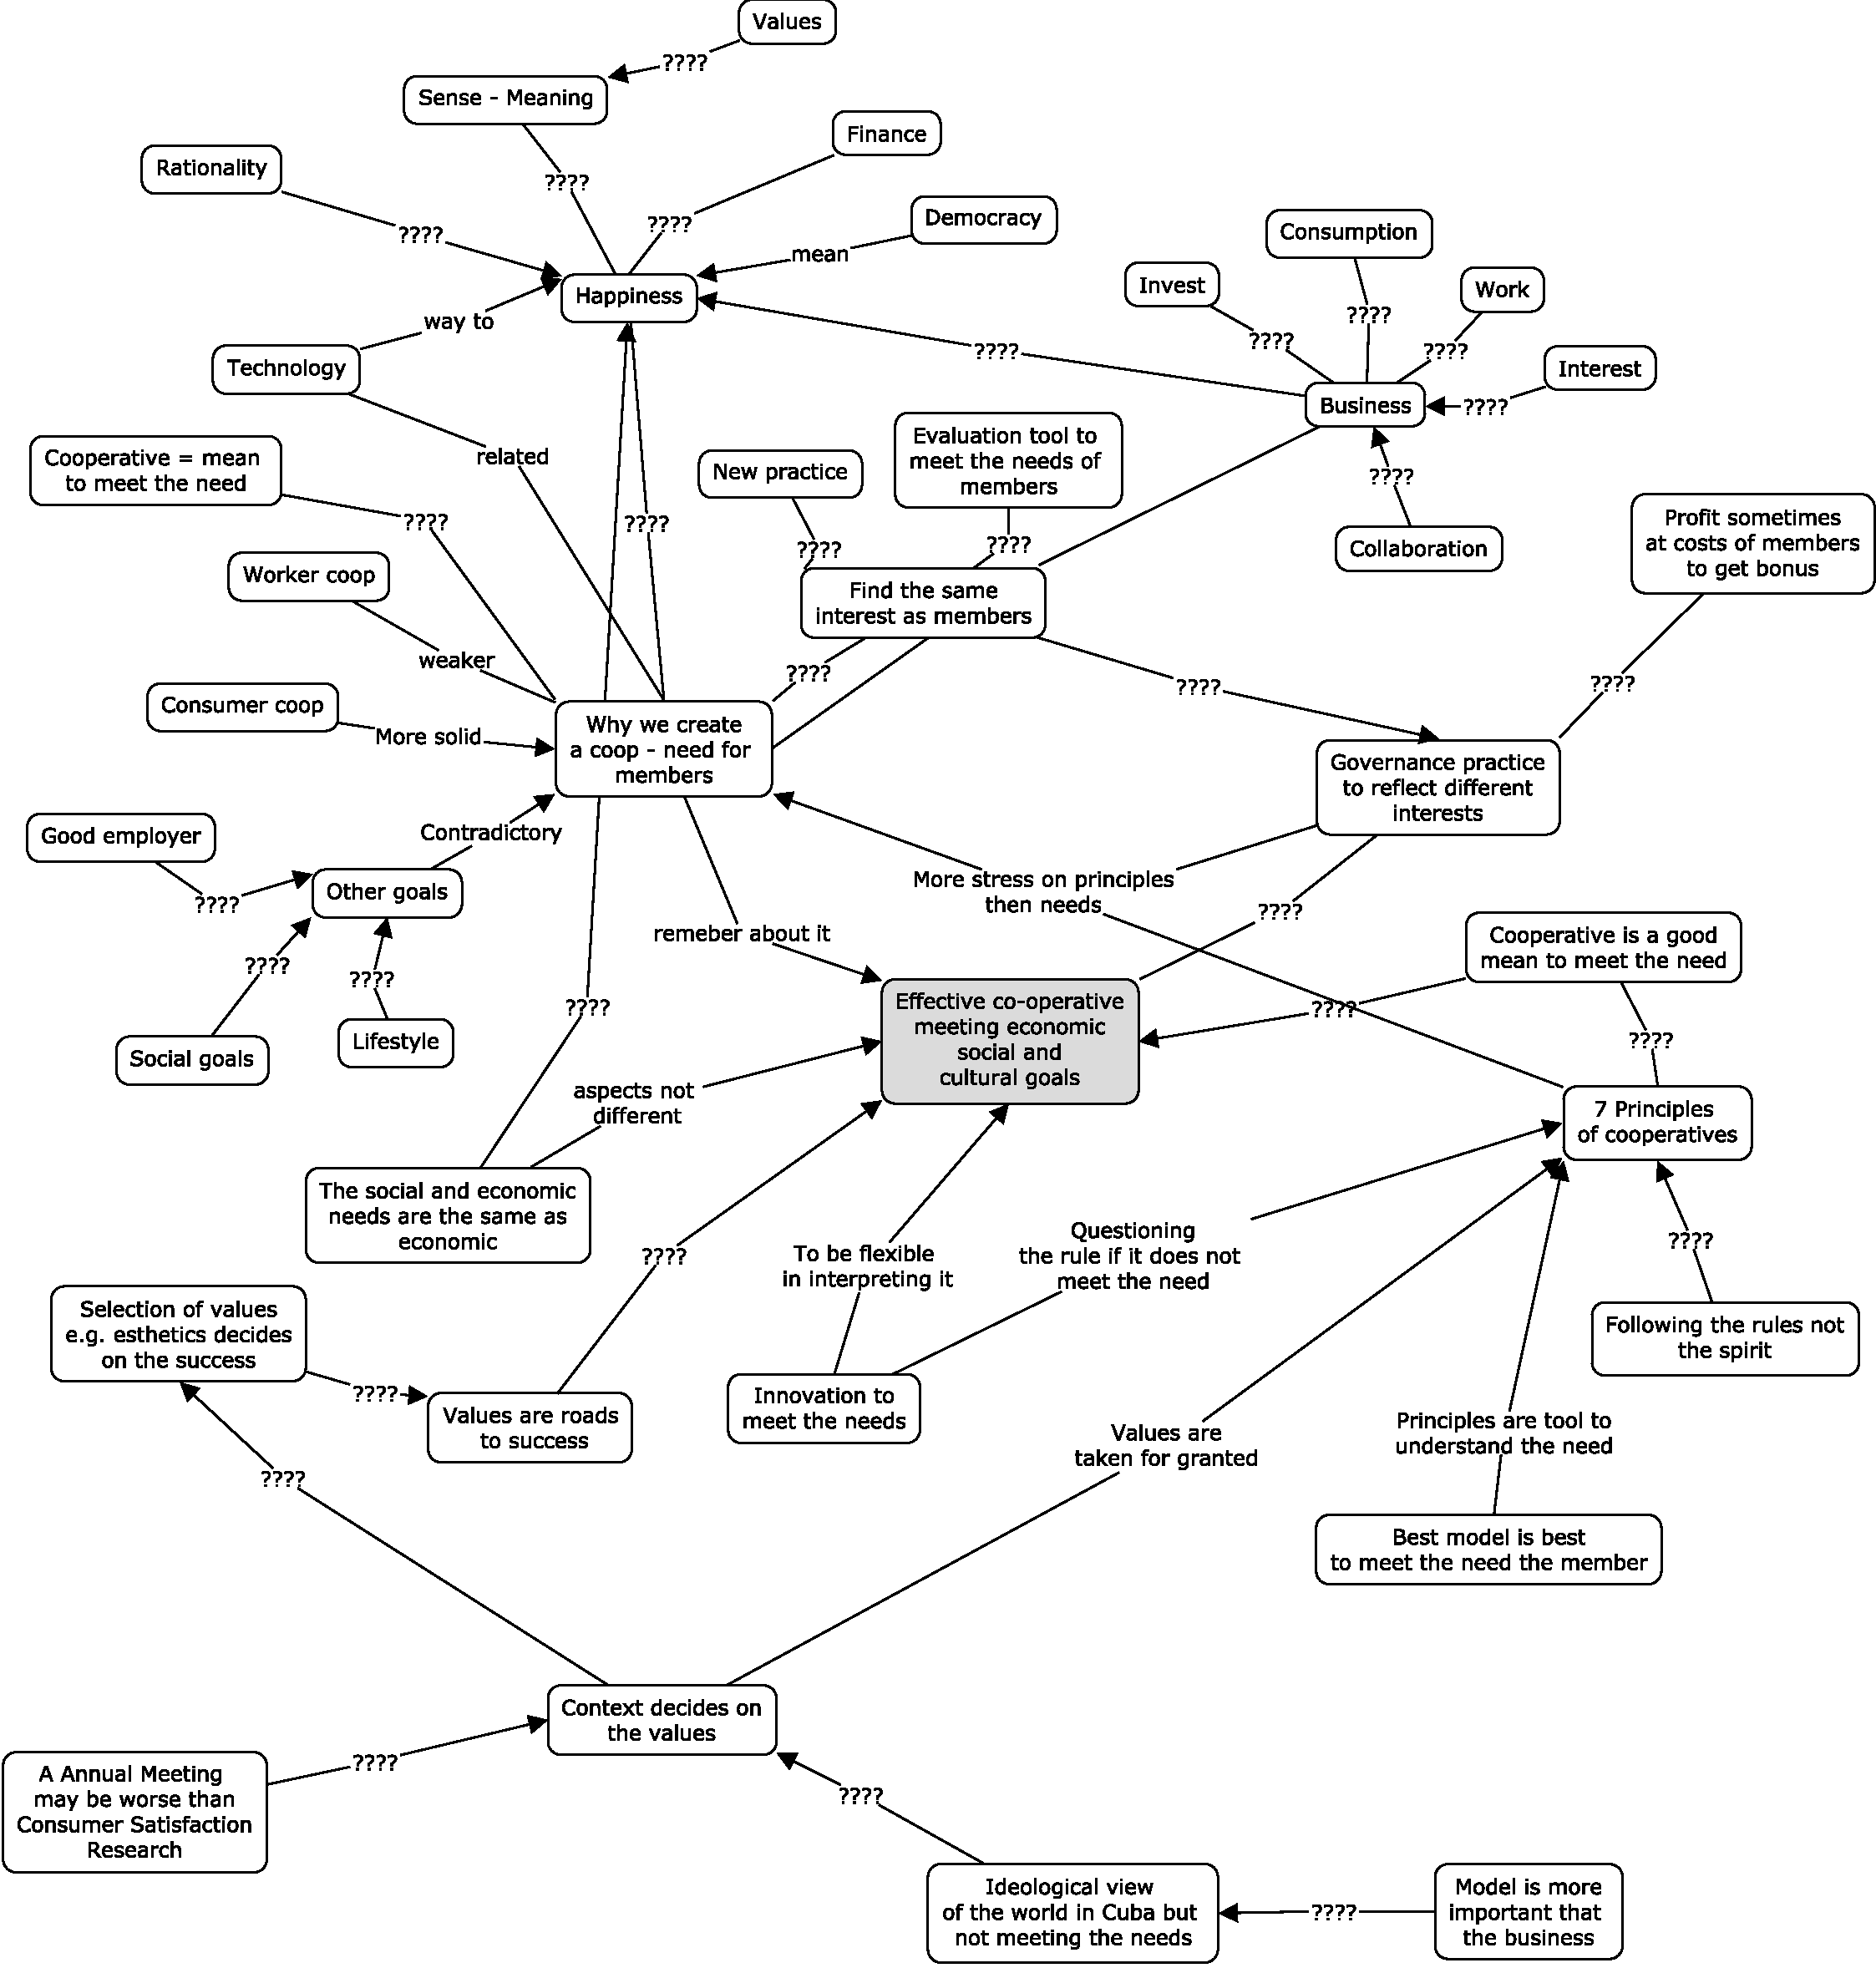
\includegraphics[width=1.2\textwidth]{ART_Bielecki/fig6.pdf}%
 \end{adjustwidth}
 \end{center}%
 \caption{An expert map of an effective coopertive 
 %\label{ref:RNDRQ89DmmkM0}(Stocki, submitted).
 \parencite[][]{stocki_tacit_nodate}.}\label{bie:fig4}
\end{figure}




The concept of structural information, and particularly its analytic opportunities related to balls of different diameter might allow focus on such a~huge 410 
%\label{ref:RNDn7F9scOnGs}(Iasiello et al., 2023)
\parencite[][]{iasiello_whats_2023} %
 or 40 elements map in Fig.4 without the necessity to synthesize it.



\subsection{Application the concept of structural information to cognitive maps}



How people think in the economic context, and particularly in management has a~direct impact on companies' success. No wonder, management is one of the domains that uses the tool such as map analysis most often. Preliminary results indicate that managers' cognitive maps, may impact the decision making process and, as a~result, success of a~company. Thus, investigation of the structure and complexity of such maps can be in such sort of studies in psychology of management. The example of cognitive maps obtained during these studies is presented in Fig.5. The managers were asked of drawing cognitive maps on which the notion \textit{responsibility} was the starting point. On the cognitive map it was necessary to place all the concepts that the concept of \textit{responsibility} affects or which have an impact on \textit{responsibility}. It was also necessary to take into account the mutual influence of the placed concepts.



The presented concept of information, at its current, initial stage, is not a~powerful enough tool to study the structure of natural language utterances, much less the meaning of utterances. Nevertheless, it is sufficient to study the structure of cognitive maps without analyzing their lexical content. Let us consider two cognitive maps obtained during the investigations described in subsection 4.1 presented in Fig.5. The arrows on the cognitive maps means that \textit{notion A~affects notion B.} This is a~relation in the sense of the concept of structural information. The graphs generated by the said relation generates the graphs shown in Fig.6. The filled nodes correspond to the utterance \textit{responsibility}, that was the starting point of the studies.

\begin{figure}[htbp]
\begin{adjustwidth}{-.1\textwidth}{}
  \begin{minipage}{.5\linewidth}
    \centering
  \begin{tikzpicture}[scale=0.6, transform shape,
   centernode/.style={ellipse, align=center, minimum width=2cm},
        mynode/.style={draw, align=center, rounded corners, minimum width=1cm, minimum height=0.5cm},
        myarrow/.style={<-, >=latex, thick},
        node distance=1cm and 2cm
    ]
    
    \node[centernode] (responsibility) {Responsibility};
    \node[mynode, above left=of responsibility, xshift=1.5cm] (submission) {Submission to\\ supervisors};
    \node[mynode, above right=of responsibility, xshift=-1cm] (decision) {Decision\\ making};
    \node[mynode, below right=of responsibility,yshift=.5cm, xshift=-.7cm] (action) {Action};
    \node[mynode, below left=of responsibility, yshift=1cm, xshift=.5cm] (leading) {Leading a team\\ of people};
    \node[mynode, below=of responsibility] (response) {Response to\\ problems};
    
    \draw[myarrow] (submission) -- (responsibility);
    \draw[myarrow] (decision) -- (responsibility);
    \draw[myarrow] (action) -- (responsibility);
    \draw[myarrow] (leading) -- (responsibility);
    \draw[myarrow] (response) -- (responsibility);
  \end{tikzpicture}
	\end{minipage}%
	 \begin{minipage}{.6\linewidth}
  \centering
  \begin{tikzpicture}[scale=0.6, transform shape,
   centernode/.style={ellipse, align=center, minimum width=2cm},
                  mynode/.style={draw, align=center, rounded corners, minimum width=1cm, minimum height=0.5cm},
             myarrow/.style={->, >=latex, thick},
             dbarrow/.style={<->, >=latex, thick},
             node distance=1cm and 2cm
         ]
         
         % Central node
         \node[centernode] (responsibility) {Responsibility};
         
         % Top nodes
         \node[mynode, above left=of responsibility, yshift=1cm, xshift=1cm] (loyalty) {Loyalty};
         \node[mynode, above=of responsibility, xshift=1cm] (honesty) {Honesty};
         \node[mynode, above=of honesty, xshift=1.5cm] (tolerance) {Tolerance};
         
         % Bottom nodes
         \node[mynode, below left=of responsibility,  xshift=1.5cm] (respEmployees) {Responsibility for\\ other employees};
         \node[mynode, below right=of responsibility, xshift=-.5cm] (professionalism) {Professionalism};
         
         % Draw arrows
         \draw[myarrow] (loyalty) -- (responsibility);
         \draw[myarrow] (honesty) -- (responsibility);
         \draw[dbarrow] (tolerance) -- (honesty);
         \draw[myarrow] (responsibility) -- (professionalism);
         \draw[dbarrow] (respEmployees) -- (responsibility);
         \draw[dbarrow] (respEmployees) -- (professionalism);
         \draw[dbarrow] (honesty) -- (professionalism);
         \draw[dbarrow] (tolerance) -- (professionalism);
  \end{tikzpicture}
\end{minipage}
\end{adjustwidth}
 \caption{Examples of two cognitive maps obtained during investigations described in subsection 4.1.}
 \label{fig:maps}
\end{figure}
\begin{figure}[htbp]
 \centering % Center the figure content

 % First subfigure
 \begin{minipage}[b]{.4\textwidth}
   \centering
   \includegraphics[width=\textwidth]{ART_Bielecki/fig9.png}
   \subcaption{Graph \textit{G}\textit{\textsubscript{1}}}
 \end{minipage}%
 \hfill
 \begin{minipage}[b]{.53\textwidth}
   \centering
   \includegraphics[width=\textwidth]{ART_Bielecki/fig10.png}
   \subcaption{Graph \textit{G}\textit{\textsubscript{2}}}
 \end{minipage}
 \caption{The structure of cognitive maps presented in Fig.5. The numbers in parentheses in graph G\textsubscript{2} denote indegree and outdegree of the node.}
 \label{bie:fig6}
\end{figure}




Let us consider graph \textit{G}\textit{\textsubscript{1}} presented in Fig.6(a). It consists of six nodes and five edges, thus---see formulae (1) and (3) we have
\[
H^{\textit{ndex}} = \log 7 \approx 2.8,
\]
\[
H^{\textit{edex}} = \log 6 \approx 2.6.
\]

The filled node is distinguishable from any other whereas the others are pairwise indistinguishable. Thus, on the set of the nodes we have partition \textit{(5,1)} (in the Hellerman sense) and, as a~consequence
\[
H^{\textit{node}} = -6 \left[ \left(\frac{5}{6}\right) \log\left(\frac{5}{6}\right) + \left(\frac{1}{6}\right) \log\left(\frac{1}{6}\right) \right] \approx 3.9.
\]

It is obvious that all edges are pairwise indistinguishable, so
\[
H^{\textit{edge}} = 0.
\]

Graph \textit{G}\textit{\textsubscript{2}} consists of six nodes and thirteen edges, so
\[
H^{\textit{ndex}} = \log 7 \approx 2.8,
\]
\[
H^{\textit{edex}} = \log 13 \approx 3.7.
\]

In graph \textit{G}\textit{\textsubscript{2}} each two nodes are distinguishable. Indeed, apart from two nodes, all others have pairwise different bi-labels that encoded indegree and outdegree of the node---see Fig.6(b). Thus, they are pairwise distinguishable. Two nodes that have bi-label \textit{(2,2)} are also distinguishable because the node-balls of radius \textit{1} and centers at these points are not isomorphic. The one of two node-balls is a~subgraph that consists of the nodes labeled as \textit{(2,2), (3,4), (2,3)} and six edges connecting them. The second one consists of the nodes labeled as \textit{(2,2), (3,4), (3,2)} and five edges connecting them. Since the numbers of edges in two these balls are different, the node-balls are not isomorphic. As a~consequence, the partition in the Hellerman sense of the set of nodes is \textit{(1,1,1,1,1,1)} and
\[
H^{\text{node}} = -6 \left[ 6 \left(\frac{1}{6}\right) \log\left(\frac{1}{6}\right) \right] \approx 15.5.
\]

In graph \textit{G}\textit{\textsubscript{2}} each pair of edges are distinguishable because for any two edges it is not true that bi-labels of the nodes from which the edges originate are equal and it is not true that bi-labels of the nodes to which the edges enters are equal. Furthermore, let us notice that in the context of the considered cognitive maps self-reference of the relation has no sense, so it is natural to assume that \textit{M=n(n-1)=6·5=30.} So, we have a~partition in the sense defined in 
%\label{ref:RNDYnS0vMCERo}(Bielecki and Schmittel, 2022)
\parencite[][]{bielecki_information_2022} %
 equal to \textit{(1,1,1,1,1,1,1,1,1,1,1,1,1)(30)} and, as a~consequence,
\[
H^{\text{edge}} = -13 \left[ 13 \left(\frac{1}{30}\right) \log\left(\frac{1}{30}\right) \right] \approx 27.7.
\]

Thus, graphs \textit{G}\textit{\textsubscript{1}} and \textit{G}\textit{\textsubscript{2}} have the same amount of node existential information. Graph \textit{G}\textit{\textsubscript{2}} has, however, significantly more amount of edge existential information---\textit{3.7} bites versus \textit{2.6} bites. Furthermore, amount of structural information is far more greater in graph \textit{G}\textit{\textsubscript{2}}---\textit{15.5} versus \textit{3.9} bites in the case of node structural information and \textit{27.7} versus \textit{0} bites in the case of edge structural information.



As it has been mentioned, at the current stage of studies it is impossible to conduct deep lexical analysis in the frame of the proposed concept. Nevertheless, labeling could be introduced to distinguish the central term in the analyzed maps---\textit{responsibility---}from the other terms. In the case of two analyzed maps, however, such labeling does not provide any additional information. In fact, in the case of graph \textit{G}\textit{\textsubscript{1}} it would distinguish the central notion from the other ones, but it is already distinguished with the partition of the set of the nodes introduced by the considered relation. In the case of graph \textit{G}\textit{\textsubscript{2}} all nodes are distinguishable by the considered relation.



It should be stressed that in the context of structural information, labeling is not arbitrary, but encodes information about the nature of the elements of the base set. Labeling by the common label the atoms of the same chemical elements is a~typical example 
%\label{ref:RNDizAbmzmYKf}(see Bielecki and Schmittel, 2022).
\parencite[see][]{bielecki_information_2022}. %
 In this paper, in the analyzed cognitive maps, the term \textit{responsibility} is highlighted as the base term provided by the researcher to which referred all other terms used by the person being examined. Therefore, without falling into the trap of lexical meaning, it was proposed to label this word with a~unique label as a~concept having a~unique status in the study. The remaining vertices were labeled with a~different label, but all with the same one. This labeling was done in order to distinguish the base term without going into lexical analysis.



\section{Concluding remarks}

Let us summarize the proposed concept of information and the presented example of its application. The concept of information at the current stage of the studies is formulated in purely mathematical way. The definitions of various types of information have been put forward and their basic properties have been specified. This was done with care for formal correctness and completeness. Although the concept was originally dedicated to applications for analysis of biological structures and processes 
%\label{ref:RNDIJr53JnJPy}(see Bielecki, 2015)
\parencite[see][]{bielecki_general_2015} %
 and was preliminary tested by using to analysis of molecular cybernetics 
%\label{ref:RNDBmHEi1m1dC}(see Bielecki and Schmittel, 2022)
\parencite[see][]{bielecki_information_2022} %
 it turned out that the concept is also applicable to analysis of cognitive maps. As for the analyzed example of applications, formal analysis of such maps with the assistance of structural information concept allows the researchers to go beyond from the simple analysis of the map content to the analysis of the maps structure and complexity. As is visible in the example above, we can, for instance, analyze the role of the central concept of responsibility in detail showing that in the first map if removed, it disintegrates the structure of the whole graph, whereas the same removing of the central concept from the second graph causes only partial disintegration of the structure of the graph. This means that in critical moments in the decision making process, when some important aspect is undermined, the first manager may have no indication how to behave whereas the second one may reconstruct the decision with the help of a~substitute. Such formal analysis of the concepts make visible properties of our thinking that were, so far, treated as tacit. Furthermore, the proposed approach allow the researcher to calculate precisely amount of information in the cognitive maps.



\end{artengenv2auth}

